\chapter{External specification}


After running the presented program, the end user will see a window with a graph and a list from which it is possible to choose the company the user would like to investigate. There is a graph presented in the main window that consists of two lines - red and blue. The blue line represents real prices that can be read from the stock market, and the red line represents the predicted prices provided by the neural network. At the bottom of the screen, there is a list of companies. By changing the company on the list, the graph will change accordingly.
Changing the options for the neural network in variables.py file is possible. All the variables used in the project can be changed as the end user wants. The things that could be changed are the type of the reading price (can be open price, closing price, the highest price, the lowest price or volume of the stocks traded), the number of epochs in training the neural network, start date, end date, and the interval (can be daily, weekly or monthly), and size of the input data.
It is also possible to load the neural network model instead of training a new one by uncommenting the load model function in hortus.py and placing one of the eight models' names in it.

 
\begin{figure}
\centering
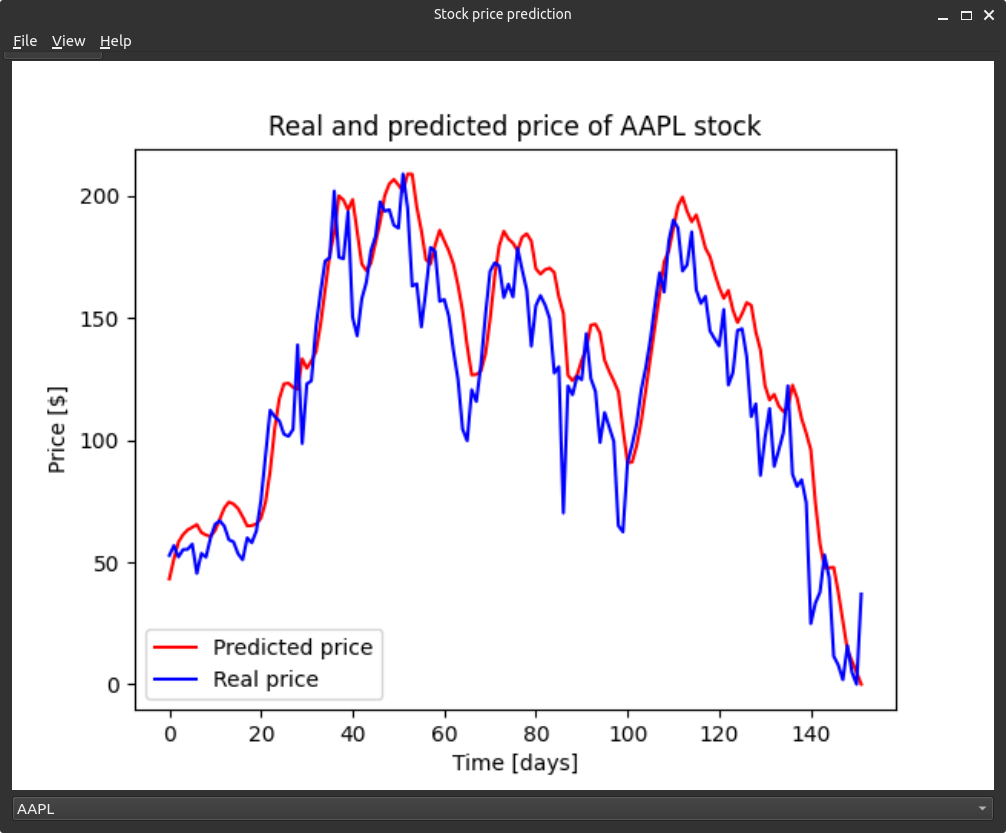
\includegraphics[width=0.5\textwidth]{./graf/MainWindow.png}
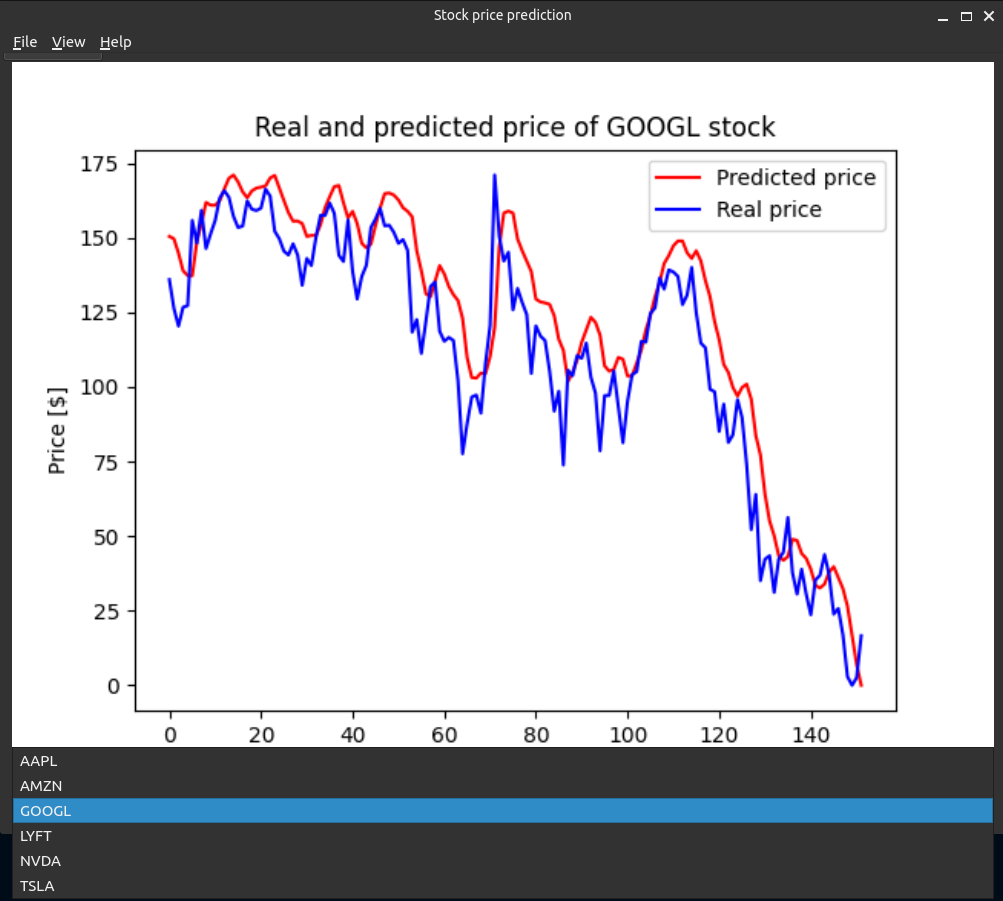
\includegraphics[width=0.5\textwidth]{./graf/MainWindow_select.png}
\caption{Main window of stock price prediction project.}
\label{fig:label}
\end{figure}

\clearpage
\begin{figure}
\centering
\begin{lstlisting}
    # Variables
    # company_name = 'AAPL' # company NASDAQ name
    price_type = 'open' # open, close, high, low, volume
    epochs = 15

    # Time interval
    startDate = '2021-06-01'
    endDate = '2022-06-01'
    interval = 'daily' # daily, weekly or monthly

    # Shape of input data
    chunkSize = 100

    # Company name dict
    company_name = ['AAPL', 'AMZN', 'GOOGL', 'LYFT', 'NVDA', 'TSLA']
\end{lstlisting}
\caption{Neural network's parameters.}
\label{fig:pseudocode:listings}
\end{figure}

%%%%%%%%%%%%%%%%%%%%%
% FIGURE FROM FILE
%
%\begin{figure}
%\centering
%
\includegraphics[width=0.5\textwidth]{./graf/politechnika_sl_logo_bw_pion_en.pdf}
%\caption{Caption of a figure is always below the figure.}
%\label{fig:label}
%\end{figure}
%Fig. \ref{fig:label} presents …
%%%%%%%%%%%%%%%%%%%%%
%
%%%%%%%%%%%%%%%%%%%%
%% SUBFIGURES
%
%\begin{figure}
%\centering
%\begin{subfigure}{0.4\textwidth}
%    
\includegraphics[width=\textwidth]{./graf/politechnika_sl_logo_bw_pion_en.pdf}
%    \caption{Upper left figure.}
%    \label{fig:upper-left}
%\end{subfigure}
%\hfill
%\begin{subfigure}{0.4\textwidth}
%    
\includegraphics[width=\textwidth]{./graf/politechnika_sl_logo_bw_pion_en.pdf}
%    \caption{Upper right figure.}
%    \label{fig:upper-right}
%\end{subfigure}
%
%\begin{subfigure}{0.4\textwidth}
%    
\includegraphics[width=\textwidth]{./graf/politechnika_sl_logo_bw_pion_en.pdf}
%    \caption{Lower left figure.}
%    \label{fig:lower-left}
%\end{subfigure}
%\hfill
%\begin{subfigure}{0.4\textwidth}
%    
\includegraphics[width=\textwidth]{./graf/politechnika_sl_logo_bw_pion_en.pdf}
%    \caption{Lower right figure.}
%    \label{fig:lower-right}
%\end{subfigure}
%        
%\caption{Common caption for all subfigures.}
%\label{fig:subfigures}
%\end{figure}
%Fig. \ref{fig:subfigures} presents very important information, eg. Fig. \ref{fig:upper-right} is an upper right subfigure.
%%%%%%%%%%%%%%%%%%%%%
